\documentclass[twoside,11pt]{homework}

\coursename{Unsupervised Learning (2018 Fall)} 

\studname{Youki Cao}    % YOUR NAME GOES HERE
\studmail{}% YOUR UNI GOES HERE
\hwNo{2}                   % THE HOMEWORK NUMBER GOES HERE
\date{Oct 26 2018} % DATE GOES HERE

% Uncomment the next line if you want to use \includegraphics.
%\usepackage{graphicx}

\begin{document}
\maketitle

\section*{Problem 1}
\begin{enumerate}
    \item\textbf{ "A lower bound on the distortion of embedding planar metrics into Euclidean space" by Newman and Rabinovich.}
    \newline
    In general this paper gives a tight lower bound on the distortion of embedding planar metrics into Euclidean spaces. For definition, a metric is called planar if it can be obtained by restricting the geodetic metric of some weighted planar graph to a subset of its vertices. Also given two metric spaces $(S,\mu),(R,\delta)$ and an embedding $f: S \rightarrow R$, define the distortion of $f$ as the product of the max expansion and the max contraction of $f$, which can be proved to be great or equal to 1, and comes to be 1 iff $f$ preserves $\mu$ up to scaling.
    $$distr(f)=\underset{x,y \in S}{\max}\frac{\delta(f(x),f(y))}{\mu(x,y)} \underset{x,y\in S}{\max} \frac{\mu(x,y)}{\delta(f(x),f(y))}$$
    For a finite metric $\mu$, define $c_2(\mu)$ and $c_1(\mu)$ respectively as the smallest possible distortion of embedding $\mu$ into real Euclidean and $l_1$ space. It holds that $c_2(\mu) \geq c_1(\mu)$. So now we want to establish a lower bound for series-parallel metrics.
    \begin{figure}[]
    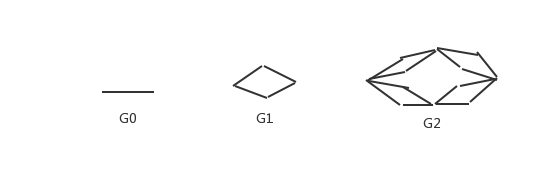
\includegraphics[height=6.0cm]{graph.png}
    \caption{The graph of $G_0,G_1,G_2$}
    \end{figure}
    Define a family $\{G_k\}$ as below: $G_0$ is a single edge. $G_i$ is generated by replacing each edge of $G_{i-1}$ by two parallel paths, each containing two edges. The length of every edge in $G_i$ is defined as $2^{-i}$, half of that in $G_{i-1}$. The sketch of graph $G_1,G_2,G_3$ is shown in Figure 1. Also we define anti-edge as below: assume we replace the edge $(a,b)$ in $G_i$ with edges $(a,x), (x,b), (a,y), (y,b)$, then we call the pair vertices $\{x,y\} \subset V(G_i)$ the anti-edge of $(a,b)$. It's easy to notice that $G_k$ is a series-parallel graph containing $4^k$ edges and $(2*4^k+4)/3$ vertices. Then it comes to our main theorem.
    
    \begin{theorem}
    Let $\mu$ denote the geodetic metric of $G_k$. Then we have $c_2(\mu) \geq \sqrt{k+1}$.
    \end{theorem}
    I provide the proof sketch here. Let $f:V(G) \rightarrow \mathcal{R}^d$ be an embedding of $\mu$ into Euclidean space. Assume that $f$ is non-expanding. Let $\alpha=min_{v,u \in V(G_k)}(||f(v)-f(u)||_2/\mu(v,u))$. All we need to do is to show $\alpha \leq \frac{1}{\sqrt{k+1}}$. Firstly we use downwards induction to prove that for any$(a,c) \in E(G_i)$,
    $$||f(a)-f(c)||_2 \leq \sqrt{1- (k-i)\alpha^2}\mu(a,c)$$ The induction can be proved using the fact that for any four points $a,b,c,d$ in Euclidean space the sum of the squares of the diagonals will not exceed the sum of the squares of the sides. Use it to the anti-edge and the original edges, we can get the induction proved. Then we consider the edge $(s,t)$ of $G_0$. The images of $s$ and $t$ are at least $\alpha$ and at most $\sqrt{1-k\alpha^2}$ apart. We we have $\alpha \leq 1/\sqrt{k+1}$. Therefore proved.
    Furthermore we can slightly strengthen the theorem by restoring all pairs edges. Let $H_0$ consist of single edge of length 1, and let $H_i$ be obtained by taking $H_{i-1}$. In addition to existing vertices and edges, introducing for each edge $e=(a,c)$ of $H_{i-1}$ of length $2^{-(i-1)}$ two new vertices $b_e,d_e$, a new edge $(b_e,d_e)$ of length $2^{-(i-1)}$ and four new edges $(a,b_e), (b_e,c), (c,d_e),(d_e,a)$ and each of length $2^{-i}$. $H_{i-1}$ isometrically embeds into $H_i$ under the natural identification of the vertices. Also by the preceding discussion we have theorem 2.
    
    \begin{theorem}
    In any embedding $f$ of $H_k$ into Euclidean space which does not expand the edges, there exists an edge in $E(H_k)$ whose length is contracted by $f$ by at least a factor of $\sqrt{k+1}$.
    \end{theorem}
    
    
    \item
    \textbf{"On the Impossibility of Dimension Reduction in $l_1$" by Brinkman and Charikar.}
    
    This paper shows strong lower bounds for general dimension reduction in $l_1$. It gives an explicit family of $n$ points in $l_1$ such that any embedding with distortion $\delta$ requires $n^{\Omega(1/\delta^2)}$ dimensions. So there is no analog of the JL Lemma for $l_1$.
    
    We first define the concept of stretch-limited embedding. Suppose a metric space $(M,\rho)$ could be written as a collection of $t$ line metrics $\{\rho_{1}, \cdots, \rho_{t}\}$ with weights $\{\omega_{1}, \cdots, \omega_{t}\}$ s.t. the sum is equal to $1$. Define the weighted distance function $d'$ as:
    \begin{align*}
        d'(u,v) = \sum\limits_{i=1}^{t}\omega_{i}|\rho_{i}(u)-\rho_{i}(v)|
    \end{align*}
    Then we focus on series-parallel graphs called recursive diamond graphs the same as the previous paper. A vertex is said to have \textit{level} $k$ if it first appears in the order $k$ graph but not in the order $k-1$ graph. The two new vertices created by replacing an edge with a diamond are called siblings and they are called the diagonal of that specific diamond. We'll call a diagonal \textit{level} $k$ if the vertices concerned are \textit{level} $k$. For a label $x$, $e_{x}$ denotes the edge labeled as $x$, $f_{x}$ denote the diagonal whose label is $x$. This leaves the original first edge unlabeled. We will treat it as if being "diagonal like" and refer to as $f_{*}$. The length of a particular edge labeled as $x$ is denoted as $m_{x}$.The length of a diagonal labeled $y$ is denoted as $d_{y}$. For the original first edge, $d_{*}$. For each edge, the two endpoints are designated as \textit{hd} and \textit{tl}, so we can obtain an expression $\rho(hd(e))-\rho(tl(e))$. For a diagonal edge $e_{y}$ the two endpoints are designated as \textit{tp} and \textit{bt}, such that $\rho(tp(e_{y})) \geq \rho(bt(e_{y}))$ and denote the length of that diagonal edge as $d_{y}$. We can define the following
    \begin{align*}
    m_{x} =& \rho(hd(e_{x})) - \rho(tl(e_{x}))\\
    d_{x} =& \rho(tp(f_{x})) - \rho(bt(f_{x}))\\
    n_{x} =& \frac{\rho(tp(f_{x}))+\rho(bt(f_{x}))}{2} - \frac{\rho(hd(e_{x})) + \rho(tl(e_{x}))}{2}
    \end{align*}
    From all these definitions we can calculate $m_{x0},m_{x2},m_{x3}$, and find a representation of $m_x$ as below:
    \begin{align*}
    m_{x} = \frac{d_{*}}{2^{|x|}} + \sum\limits_{y \sqsubset x}\frac{S(x_{|y|+1})d_{y}}{2^{|x|-|y|}} + \sum\limits_{y \sqsubset x} \frac{T(x_{|y|+1})n_{y}}{2^{|x|-|y|-1}}
    \end{align*}
    Then we will place our edges and diagonals into groups and write the constraints in terms of the average distances in these groups. We group edges into $2^{k}$ edges, where each group is identified by label $\{0,1\}^{k}$. An edge $e_{x}$ is in group $z \in \{0,1\}^{k}$ if $x (mod 2) = z$. Similarly diagonals of level $i$ are grouped into $2^i$ groups, identified with labels in $\{0,1\}^i$.
    $$\overline{m_{z}} = \frac{1}{2^{k}} \sum\limits_{x:x(mod)2 = z}|m_{x}|$$
    $$\overline{d_{z}} = \frac{1}{2^{k}}\sum\limits_{x:x(mod)2 = z} d_{x}$$
    So we can rewrite our $\delta$ constraint.
    $$\delta (\overline{d_{*}} + \sum\limits_{i=0}^{k-1}\sum\limits_{y \in \{0,1\}^{i}}\overline{d_y}) - \gamma \sum\limits_{x \in \{0,1\}^{k}} \overline{m_x} \geq k+1-\gamma$$
    For a group label $z \in \{0,1\}^k$,
    $$\overline{m_z}\geq \frac{d_{*}}{2^{k}} + \sum\limits_{y \sqsubset z} S(z_{|y|}+1)\frac{\overline{d_{y}}}{2^{k-|y|}}$$
    $$\overline{m_z}\geq -\frac{d_{*}}{2^{k}} - \sum\limits_{y \sqsubset z} S(z_{|y|}+1)\frac{\overline{d_{y}}}{2^{k-|y|}}$$
    So now we can give our linear program and construct the dual as algo 2.\\
    \begin{center}
    \begin{algorithm}[H]
    \caption{Linear Programming}
    \textbf{min} $s$
    \begin{enumerate}
      \item $\delta (\overline{d_{*}} + \sum\limits_{i=0}^{k-1}\sum\limits_{y \in \{0,1\}^{i}}\overline{d_y}) - \gamma \sum\limits_{z \in \{0,1\}^{k}} \overline{m_x} \geq k+1-\gamma$   $[\mu]$
      \item $\forall z \in \{0,1\}^{k} \quad s/2^{k} \geq \overline{m_{z}}$   $[p_{z}]$
      \item $\forall z \in \{0,1\}^{k} \quad \overline{m_{z}} \geq \frac{\overline{d_{*}}}{2^{k}} + \sum\limits_{y \sqsubset z} S(z_{|y|}+1)\frac{\overline{d_y}}{2^{k-|y|}}$   $[\alpha_{z}]$
      \item $\forall z \in \{0,1\}^{k} \quad \overline{m_{z}} \geq -\frac{\overline{d_{*}}}{2^{k}} - \sum\limits_{y \sqsubset z} S(z_{|y|}+1)\frac{\overline{d_{y}}}{2^{k-|y|}}$   $[\beta_{z}]$
    \end{enumerate}
    \end{algorithm}
    \end{center}
    \begin{center}
    \begin{algorithm}[H]
    \caption{Dual Problem}
    \textbf{max} $(k+1-\gamma)\mu$
    \begin{enumerate}
      \item $\forall z \in \{0,1\}^{k} \quad -\gamma \mu - p_z+\alpha_z+\beta_z\leq 0$   $[\overline{m_{z}}]$ 
      \item $\sum\limits_{z \in \{0,1\}^{k}}p_{z} \leq 2^{k}$   $[s]$ 
      \item $\forall y \in \bigcup_{i \in [0,k-1]}\{0,1\}^{i} \quad \mu\delta +\sum\limits_{v \in \{0,1\}^{k-|y|}}\frac{S((yv)_{|y|+1})(\alpha_{yv}-\beta_{yv})}{2^{k-|y|}} \leq 0$   $[\overline{d_{y}}]$ 
      \item $\mu\delta + \sum\limits_{z \in \{0,1\}^{k}}\frac{\alpha_{z}-\beta_{z}}{2} \leq 0$   $[\overline{d_{*}}]$
    \end{enumerate}
    \end{algorithm}
    \end{center}
    Finally we can get the solution. Then for any $n$ arbitrary points with $l_{1}$ metric, we can construct a similar structure analogous to the recursive diamond graph. Starting from the original first edge with endpoints $0$ and $1$, the vertices will correspond to points in $\{0,1\}^{i}$. To go from level $i$ to $i+1$, first double the dimensions. Then replace the parent node $x$ and $y$ with $xx$ and $yy$. The children will be the points $xy$ and $yx$. The level $k$ recursive diamond graph corresponds to a set of $\Theta(4^{k+1})$ points in $2^{k+1}$ dimensions. Therefore the $n$ points could be embedding into a space with dimension $n^{\Omega(1/\delta^{2})}$ with the distortion $\delta$. So the dimensional reduction in $l_{1}$ without distortion is impossible.  

\end{enumerate}

\section*{Problem 2}
\subsection*{(a)}

From definition we know $G = -\frac{1}{2}H^\mathbf{T}DH$. Here $H$ is a symmetric matrix, so that $H^\mathbf{T}=H$. Because 
\[H_{ij}=\begin{cases}

1-\frac{1}{n}&\text{$i = j$},\\

-\frac{1}{n}&

\text{$i \neq j$}.

\end{cases}\]
So we have
\begin{align*}
    G_{ij} / (-\frac{1}{2})&= \sum_{l=1}^n \sum_{k=1}^n H_{il}\rho_{lk}H_{kj}\\
    &=(1-\frac{1}{n})^2 \rho_{ij} + 
    \sum_{k \neq j}(1-\frac{1}{n})(-\frac{1}{n})\rho_{ik} +
    \sum_{l\neq i}(1-\frac{1}{n})(-\frac{1}{n})\rho_{lj} +
    \sum_{l \neq i}\sum_{k\neq j}\frac{1}{n^2}\rho_{lk}\\
    &=\rho_{ij} - \frac{2}{n}\rho_{ij} + \frac{1}{n^2}\rho_{ij} - \frac{1}{n} \sum_{k \neq j}\rho_{ik} + \frac{1}{n^2}\sum_{k \neq j}\rho_{ik} -
    \frac{1}{n} \sum_{l\neq i}\rho_{lj} + \frac{1}{n^2}\sum_{l\neq i}\rho_{lj} + 
    \sum_{l \neq i}\sum_{k\neq j}\frac{1}{n^2}\rho_{lk}\\
    &= \rho_{ij} - \frac{1}{n}\sum_{k=1}^n \rho_{ik} - \frac{1}{n}\sum_{l=1}^n \rho_{lj} + \frac{1}{n^2}\sum_{l=1}^n\sum_{k=1}^n\rho_{lk}\\
    &= \rho_{ij} - \frac{1}{n}\sum_{j}\rho_{ij} - \frac{1}{n}\sum_{i}\rho_{ij} + \frac{1}{n^2}\sum_{ij}\rho_{ij}
\end{align*}
Therefore, $$G_{ij} = -\frac{1}{2}(\rho_{ij} - \frac{1}{n}\sum_{j}\rho_{ij} - \frac{1}{n}\sum_{i}\rho_{ij} + \frac{1}{n^2}\sum_{ij}\rho_{ij})$$

\subsection*{(b)}
For $\forall i,j$, $\rho_{ij} = ||x_i-x_j||^2 = ||(x_i-\overline{x}) - (x_j - \overline{x})||^2 = ||x_i - \overline{x}||^2 + ||x_j - \overline{x}||^2 - 2(x_i-\overline{x})^\mathbf{T}(x_j - \overline{x})$
We can calculate each term inside the paranthesis of
\begin{align*}
    G_{ij} &= -\frac{1}{2}(\rho_{ij} - \frac{1}{n}\sum_{j}\rho_{ij} - \frac{1}{n}\sum_{i}\rho_{ij} + \frac{1}{n^2}\sum_{ij}\rho_{ij})
\end{align*}
$$\rho_{ij} = ||x_i - \overline{x}||^2 + ||x_j - \overline{x}||^2 - 2(x_i-\overline{x})^\mathbf{T}(x_j - \overline{x})$$
$$-\frac{1}{n}\sum_j \rho_{ij} = 
-\frac{1}{n}(n||x_i - \overline{x}||^2 + \sum_j ||x_j - \overline{x}||^2 - 2 \sum_j (x_i - \overline{x})^\mathbf{T}(x_j - \overline{x}))$$
$$-\frac{1}{n}\sum_i \rho_{ij} = 
-\frac{1}{n}(\sum_i ||x_i - \overline{x}||^2 + n||x_j - \overline{x}||^2 - 2 \sum_i (x_i - \overline{x})^\mathbf{T}(x_j - \overline{x}))$$
$$\frac{1}{n^2}\sum_{ij} \rho_{ij} = \frac{1}{n^2}(\sum_{ij}||x_i - \overline{x}||^2 + \sum_{ij}||x_j - \overline{x}||^2 - 2\sum_{ij}(x_i - \overline{x})^\mathbf{T}(x_j - \overline{x}))$$
Because $\sum_j(x_j - \overline{x}) = \sum_j(x_j) - n\overline{x} = 0$, we have
$$-\frac{1}{n}\sum_j \rho_{ij} = 
-\frac{1}{n}(n||x_i - \overline{x}||^2 + \sum_j ||x_j - \overline{x}||^2) = -||x_i - \overline{x}||^2 - \frac{1}{n}\sum_j ||x_j - \overline{x}||^2$$
$$-\frac{1}{n}\sum_i \rho_{ij} = 
-\frac{1}{n}(\sum_i ||x_i - \overline{x}||^2 + n||x_j - \overline{x}||^2) = -\frac{1}{n}\sum_i ||x_i - \overline{x}||^2 - ||x_j - \overline{x}||^2$$

\begin{align*}
    \frac{1}{n^2}\sum_{ij} \rho_{ij} &= \frac{1}{n^2}(\sum_{ij}||x_i - \overline{x}||^2 + \sum_{ij}||x_j - \overline{x}||^2 - 2\sum_i \sum_j(x_i - \overline{x})^\mathbf{T}(x_j - \overline{x}))\\
    &= \frac{1}{n^2} (n\sum_{i}||x_i - \overline{x}||^2 + n\sum_{j}||x_j - \overline{x}||^2)\\
    &= \frac{1}{n}\sum_{i}||x_i - \overline{x}||^2 + \frac{1}{n}\sum_{j}||x_j - \overline{x}||^2
\end{align*}

\begin{align*}
     G_{ij} =& -\frac{1}{2}(\rho_{ij} - \frac{1}{n}\sum_{j}\rho_{ij} - \frac{1}{n}\sum_{i}\rho_{ij} + \frac{1}{n^2}\sum_{ij}\rho_{ij})\\
     =& -\frac{1}{2}(||x_i - \overline{x}||^2 + ||x_j - \overline{x}||^2 - 2(x_i-\overline{x})^\mathbf{T}(x_j - \overline{x}) 
     -||x_i - \overline{x}||^2 - \frac{1}{n}\sum_j ||x_j - \overline{x}||^2\\
     &-\frac{1}{n}\sum_i ||x_i - \overline{x}||^2 - ||x_j - \overline{x}||^2
     + \frac{1}{n}\sum_{i}||x_i - \overline{x}||^2 + \frac{1}{n}\sum_{j}||x_j - \overline{x}||^2
     )\\
     =& (x_i - \overline{x})^\textbf{T}(x_j -\overline{x})
\end{align*}

\subsection*{(c)}

Given $n$ items $\gamma_i.\cdots, \gamma_n \in \Gamma$, and a (symmetric) comparison function $\rho: \Gamma \times \Gamma \rightarrow \mathbf{R}$. Define $G:=-\frac{1}{2}H^{\mathbf{T}}DH$, where $D_{ij}=\rho(\gamma_i,\gamma_j)$, and $H:=I-\frac{1}{n}\mathbf{1}\mathbf{1}^T$. We want to prove that if $G$ is positive semidefinite, then the $n$ items be can isometrically embeddable in $n$-dim Euclidean space.


\begin{lemma}
For every positive definite matrix A, there exists matrix $U$ s.t. $A = U^\mathbf{T}U$.
\end{lemma}

\begin{proof}

We'll use induction to prove the results. The base situation is when $A$'s dim is 1. It's trivial to be correct.
Then we assume that for each positive definite matrix of $n-1$ dimension, it can be decomposed as $U^\mathbf{T}U$ for some $U$.
Then consider an $n$-dimensional positive definite matrix A, write A as:
$$A=
 \left[
 \begin{matrix}
   A_1 & a \\
   a^\mathbf{T} & \alpha
  \end{matrix}
  \right]
$$
Since $A_1$ is a principle submatrix of A, we have $A_1$ is also positive definite, of dimension = $n-1$. From inductive assumption we know that there exists $U_1$ s.t. $A_1 = U_1^\mathbf{T}U_1$. And $U_1$ is invertible.
Denote $Y_1 = \left[
 \begin{matrix}
   U_1 & 0 \\
   0 & 1
  \end{matrix}
  \right]$ Then we have
$$
Y_1^{-T}AY_1^{-1}= 
\left[
 \begin{matrix}
   U_1^{-T} & 0 \\
   0 & 1
  \end{matrix}
\right]
\left[
 \begin{matrix}
   A_1 & a \\
   a^\mathbf{T} & \alpha
  \end{matrix}
\right]
\left[
 \begin{matrix}
   U_1^{-1} & 0 \\
   0 & 1
  \end{matrix}
\right]
= 
\left[
 \begin{matrix}
   I & b \\
   b^\mathbf{T} & \alpha
  \end{matrix}
\right]
$$
Here $b = U_1^{-\mathbf{T}}a$.
Consider $Y_2 = 
\left[
 \begin{matrix}
   I & b \\
   0 & 1
  \end{matrix}
\right]$, and we have
$$
Y_2^{-T}Y_1^{-T}AY_1^{-1}Y_2^{-1} = 
\left[
 \begin{matrix}
   I & 0 \\
   -b^\mathbf{T} & 1
  \end{matrix}
\right]
\left[
 \begin{matrix}
   I & b \\
   b^T & \alpha
  \end{matrix}
\right]
\left[
 \begin{matrix}
   I & -b \\
   0 & 1
  \end{matrix}
\right]
=
\left[
 \begin{matrix}
   I & 0 \\
   0 & \alpha - b^\mathbf{T}b
  \end{matrix}
\right]
$$
Because the matrix $\left[
 \begin{matrix}
   I & 0 \\
   0 & \alpha - b^\mathbf{T}b
  \end{matrix}
\right]$ and $A$ are congruent, and $A$ is positive definite, we have this matrix is also positive definite. So we know $\alpha - b^\mathbf{T}b>0$, let $\lambda^2 = \alpha - b^\mathbf{T}b$, $\lambda > 0$. Denote $Y_3 = \left[
 \begin{matrix}
   I & 0 \\
   0 & \lambda
  \end{matrix}
\right]$, so we have
$$Y_2^{-T}Y_1^{-T}AY_1^{-1}Y_2^{-1} = Y_3^\mathbf{T}Y_3$$
$$A = (Y_3Y_2Y_1)^\mathbf{T}(Y_3Y_2Y_1)$$
Denote $U = Y_3Y_2Y_1$, here we have $A = U^\mathbf{T}U$. And thus we proved the situation with $n$ dimension. Then by induction, the claim is correct.

\end{proof}

\begin{lemma}
For every positive semidefinite matrix A, there exists matrix $U$ s.t. $A = U^\mathbf{T}U$.
\end{lemma}

\begin{proof}
For any positive semidefinite matrix $A$, construct a sequence ${A_k}$, $k=1,2,\cdots$. Here $A_k:=A+\frac{1}{k}I$. Then we know $A_k$ is positive definite and $A_k \rightarrow A$ when $k \rightarrow \infty$.
From Lemma 1 we know that for each $A_k$, there exists a matrix $U_k$ s.t. $A_k=U_k^\mathbf{T}U_k$. So in operator norm we have 
$$||U_k||^2 \geq ||U_k^\mathbf{T}U_k|| = ||A_k||$$
Since the eigenvalues of $A_k$ are bounded, we get the singular values of $U_k$ are bounded. So we know $\{U_k\}$ is a bounded set in the Banach space of operators. Also the underlying space is finite dimensional. So $\{U_k\}$ is relative compact. Therefore it contains a convergent subsequence, denote as $\{U_k\}$ itself for convenience, and denote its limit as $U$. For every $x,y$,
$$(Ax,y)=(\underset{k\rightarrow \infty}{\lim}A_kx,y) = (\underset{k\rightarrow \infty}{\lim}U_k^\mathbf{T}U_k x,y) = (U^\mathbf{T}Ux,y)$$
Therefore we have $A = U^\mathbf{T}U$
\end{proof}
Since $G$ is positive semidefinite, from Lemma 2 we know that there exists $X$ s.t. $G = X^TX$, where $X = [x_1, \cdots, x_n],x_1,\cdots,x_n \in \mathbb{R}^n$. By the definition of $G$, we have $G=-\frac{1}{2}H^\mathbf{T}DH$. Denote $\overline{x}$ as the vector, element of which is the mean of each row of $X$. That is $\overline{x} = \frac{1}{n}\sum_{i=1}^n x_i=\frac{1}{n}X\mathbf{1}$.
Because $H = I - \frac{1}{n}\mathbf{1}\mathbf{1}^\mathbf{T}$, we have $H\mathbf{1} = 0$. So
$$ \mathbf{1}^\mathbf{T}X^{\mathbf{T}}X\mathbf{1} = \mathbf{1}^\mathbf{T}G\mathbf{1} =-\frac{1}{2}\mathbf{1}^\mathbf{T}H^\mathbf{T}DH\mathbf{1} = 0$$
Therefore $(X\mathbf{1})^\mathbf{T}(X\mathbf{1}) = 0$. That is, $(n\overline{x})^{\mathbf{T}}(n\overline{x})=0$. So $\overline{x}=0$.
From the question 2(a), we have
\begin{align*}
    ||x_i-x_j||_2^2 =& x_i^\mathbf{T}x_i + x_j^\mathbf{T}x_j - 2x_i^\mathbf{T}x_j\\
    =& G_{ii} + G_{jj} - 2G_{ij}\\
    =& -\frac{1}{2}(\rho_{ii} - \frac{1}{n}\sum_{l}\rho_{il} - \frac{1}{n}\sum_{k}\rho_{ki} + \frac{1}{n^2}\sum_{kl}\rho_{kl})\\
    &-\frac{1}{2}(\rho_{jj} - \frac{1}{n}\sum_{l}\rho_{jl} - \frac{1}{n}\sum_{k}\rho_{kj} + \frac{1}{n^2}\sum_{kl}\rho_{kl})\\
    &+(\rho_{ij} -  \frac{1}{n}\sum_{l}\rho_{il} - \frac{1}{n}\sum_{k}\rho_{kj} + \frac{1}{n^2}\sum_{kl}\rho_{kl})\\
    =& \frac{1}{2n}(-\sum_l \rho_{il}+\sum_{l} \rho_{jl}+\sum_{l}\rho_{li}-\sum_l \rho_{lj})+\rho_{ij}\\
    =&\rho_{ij}
\end{align*}
So we have the $X$ we get can recover the Euclidean representation of the given $n$ items. \#

\section*{Problem 3}

Given two metric spaces $X = (\mathbb{R}^d, ||\cdot||_2)$ and $Y = (\mathbb{R}^{2^d}, ||\cdot||_\infty)$. We need to find an isometric embedding $\phi: X \rightarrow Y$. For a decimal based number $x$, denote its binary number as $\hat{x}$. Also denote $\hat{x}_i$ as the $i_{th}$ digit of $\hat{x}_i$. $\hat{x}_i \in \{0,1\}$.
Define $\phi$ as below: $\forall x=(x^1, \cdots, x^d) \in \mathbb{R}^d$, $\phi(x) = (y^0, \cdots, y^{2^d-1})$, where $y^l = \sum_{i:\hat{l}_i=1}x^i - \sum_{i:\hat{l}_i=0}x^i$. Because $l \leq 2^d-1$, we know the length of its binary number is at most $d$. Here if the length of its binary number is less than $d$, then we add 0 in the front so that each binary number's length is $d$. So $\phi$ is defined well. Then I'll show that $\phi$ is an isometric embedding. $\forall x_1=(x_1^1,\cdots,x_1^d),x_2 = (x_2^1,\cdots,x_2^d) \in \mathbb{R}^d$, denote $\phi(x_1) = (y_1^0, \cdots,y_1^{2^d-1}), \phi(x_2) = (y_2^0, \cdots,y_2^{2^d-1})$.
\begin{enumerate}
    \item First I will show $||\phi(x_1)-\phi(x_2)||_\infty \leq ||x_1-x_2||_1$.
    
    $\forall 0 \leq l \leq 2^d-1$, 
    \begin{align*}
        |y_1^l-y_2^l| =& |(\sum_{i:\hat{l}_i=1}x_1^i - \sum_{i:\hat{l}_i=0}x_1^i) - (\sum_{i:\hat{l}_i=1}x_2^i - \sum_{i:\hat{l}_i=0}x_2^i)|\\
        \leq & \sum_{i:\hat{l}_i=1}|x_1^i-x_2^i| + \sum_{i:\hat{l}_i=0}x_2^i|x_1^i-x_2^i|\\
        \leq& \sum_{i=1}^d |x_1^i-x_2^i|
        =||x_1-x_2||_1
    \end{align*}
    Because $l$ is randomly selected, we know that it holds for every $l$. So
    $$||\phi(x_1)-\phi(x_2)||_\infty = \underset{l}{\max} |y_1^l-y_2^l| \leq ||x_1-x_2||_1$$
    
    
    \item Then I'll show $||\phi(x_1)-\phi(x_2)||_\infty  \geq ||x_1-x_2||_1$.
    
    Denote $A_1 = \{i: x_1^i \geq x_2^i\}$, and $A_2 = \{i: x_1^i < x_2^i\}$. Find $0 \leq l \leq 2^d - 1$ so that $l=\sum_{j \in A_1}2^{d-j}$. So we have $\{i: \hat{l_i}=1\} = A_1$ and $\{i: \hat{l_i}=0\} = A_2$. 
    \begin{align*}
        ||\phi(x_1)-\phi(x_2)||_\infty =& \underset{t}{\max} |y_1^t-y_2^t|\\
        \geq& |y_1^l-y_2^l|\\
        =& |(\sum_{i:\hat{l}_i=1}x_1^i - \sum_{i:\hat{l}_i=0}x_1^i) - (\sum_{i:\hat{l}_i=1}x_2^i - \sum_{i:\hat{l}_i=0}x_2^i)|\\
        =& |\sum_{i \in A_1} (x_1^i - x_2^i) + \sum_{i \in A_2}(x_2^i - x_1^i)|\\
        =&\sum_{i \in A_1} (x_1^i - x_2^i) + \sum_{i \in A_2}(x_2^i - x_1^i)\\
        =&\sum_{i \in A_1} |x_1^i - x_2^i| + \sum_{i \in A_2}|x_2^i - x_1^i|\\
        =&\sum_{i=1}^d |x_1^i - x_2^i|
        =||x_1-x_2||_1
    \end{align*}

    
\end{enumerate}
So we have $||\phi(x_1)-\phi(x_2)||_\infty = ||x_1-x_2||_1$. Hence $\phi$ is a satisfying isometric embedding from $l_1^d$ to $l_\infty^{2^d}$. \#

\section*{Problem 4}
Let $(X, \rho)$ be an $n$-point metric space. Let $q = \ceil{\log n}$, recall from the theorem in the lecture we know that there exists a $O(\log (n))$-embedding $f:X \rightarrow l_\infty^d$ with $d = O(\log n n^{1/\log n} \log n)$ Because $n^{1/\log n} = e^{\frac{1}{\log n}\log n}=O(1)$, so we know $d=O(\log^2 n)$.
From the definition of $D$-embedding we know that $\exists r>0,\forall x,x' \in X$,
\begin{equation}
    r\rho(x,x') \leq ||f(x)-f(x')||_\infty \leq O(\log n)r \rho(x,x')
\end{equation}
Now recall question 1.2 (c) and (d) in HW0, we know that $\forall x \in \mathbb{R}^d,p=2,q=\infty$, we have
\begin{equation}
    ||x||_\infty \leq ||x||_2 \leq ||x||_\infty \cdot d^{1/2} = ||x||_\infty \cdot O(\log n)
\end{equation}
From (1) and (2) we can get, 
\begin{align*}
    r\rho(x,x') &\leq ||f(x)-f(x')||_\infty \leq ||f(x)-f(x')||_2\\&\leq||f(x)-f(x')||_\infty \cdot O(\log n) \leq O(\log ^2 n)r\rho(x,x')
\end{align*}
So let $r$ remains the same as above, $D=O(\log^2 n)$, then for $\forall x,x' \in X$,
$$r\rho(x,x') \leq ||f(x)-f(x')||_2 \leq Dr \rho(x,x')$$
Here we get that every $n$-point metric space can be $D$-embedded into $l_2^d$, with $D=O(\log ^2 n), d = O(\log^2 n)$. \#



\section*{Problem 5}
Consider a tree $G=(V,E)$ on $n$ vertices. I'll use induction to prove that it can be isometrically embedded to $l_1^{n-1}$.

\begin{enumerate}
    \item Base: when $n=2$. Denote $V = (v_1, v_2)$. Define the embedding $\phi$ as: $\phi(v_1)=0, \phi(v_2)=\rho(v_1,v_2)$. Then we have $||\phi(v_1)-\phi(v_2)||_1=\rho(v_1,v_2)$. So $\phi$ is an isometric embedding from a two-node tree to $l_1^1$.
    
    \item Induction Hypothesis: Assume that we can isometrically embed every $(n-1)$-node tree to $l_1^{n-2}$. $(n \geq 2)$
    
    \item Induction Step: Consider $\forall$ $n$-node tree $G=(V,E)$. Remove a leaf $v \in V$ and corresponding edge $(v,u)$. Denote the remains as $G'=(V',E')$. Then we know $G'$ is connected, otherwise only $u$ can be not connected to others, so there is only one edge in $E$ connecting $u$, that is $(u,v)$, since there is only one edge connecting $v$, also $(u,v)$, we can derive that $u,v$ are not connected to other points, leading to contradiction to $G$ is a tree. Plus in $G'$, we have $|V'| = |V| - 1 = |E| - 2 = |E'| - 1$. From question 6.1 in HW1 we know that $G'$ is a tree with $n-1$ nodes.
    \newline
    From induction hypothesis we know that there exists an isometric embedding $\phi': G' \rightarrow l_1^{n-2}$. Now define embedding $\phi: G \rightarrow l_1^{n-1}$ as below:
    \begin{equation*}
    \phi(x)=\left\{
    \begin{aligned}
    &(\phi'(x), 0) & &\text{if }x \in V' \\
    &(\phi'(u), \rho(v,u))& &\text{if }x = v
    \end{aligned}
    \right.
    \end{equation*}
    Then I'll show that it's isometric.
    
    \begin{enumerate}
        \item For $x_1,x_2 \in G'$, $||\phi(x_1)-\phi(x_2)||_1 = ||(\phi'(x_1),0) - (\phi'(x_2),0)||_1 =||\phi'(x_1) - \phi'(x_2)||_1 = \rho(x_1,x_2) $. Correct.
        
        \item For $x_1 \in G'$, $x_2=v$,
        \begin{align*}
            ||\phi(x_1)-\phi(v)||_1 &= ||(\phi'(x_1),0)-(\phi'(u), \rho(v,u))||_1\\
            &= ||\phi'(x_1) - \phi'(u)||_1 + |0-\rho(v,u)|\\
            &= \rho(x_1,u) + \rho(v,u)
        \end{align*}
        
        Because $v$ is a leaf node, the only edge connecting to $v$ is $(u,v)$. The path from $x_1$ to $v$ definitely go though $u$. So the shortest path from $x_1$ to $v$ is the shortest path from $x_1$ to $u$ plus the path $u$ to $v$. That means $\rho(x_1,v) = \rho(x_1,u) + \rho(u,v)$.
        
        $$||\phi(x_1)-\phi(v)||_1 = \rho(x_1,u) + \rho(v,u) = \rho(x_1,u)$$
        
        
    \end{enumerate}
    So we know that the embedding $\phi$ is isometric. And we know the statement is true for every tree with $n$ nodes.
    
    \item Conclusion: So from induction we know that any finite tree can be isometrically embedded into $l_1$. \#
    
\end{enumerate}


\section*{Problem 6}
\begin{enumerate}
    \item 
    First I'll compute $\rho^2 (Q_d)$. Denote the vertices in $Q_d$ as $v_1,v_2, \cdots, v_{2^d}$.
    \begin{align*}
        \rho^2(Q_d) =& \sum_{e \in E} \rho(e_0-e_1)^2\\
        =& \frac{1}{2}\sum_{i = 1}^{2^d} \sum_{j: \rho(v_i,v_j)=1}\rho(v_i-v_j)^2\\
        =& \frac{1}{2}\sum_{i = 1}^ {2^d}  \sum_{j: \rho(v_i,v_j)=1} 1
    \end{align*}
    From definition, we know that $\rho(v_i,v_j)=1$ iff in $v_j$ there is exactly one coordinate different from $v_i$, so there is exactly $d$ different $v_j$ that is connected to $v_i$. So
    $$
        \rho^2(Q_d) = \frac{1}{2}\sum_{i = 1}^ {2^d}  \sum_{j: \rho(v_i,v_j)=1} 1 = \frac{1}{2}\sum_{i = 1}^ {2^d} d = 2^{d-1}d
    $$
    \newline
    Then I'll compute $\rho^2(K_{2^d})$.
    For fix $v_i$, the number of $v_j$ so that $\rho(v_i,v_j)=t$ is equal to ${d \choose t}$.
    \begin{align*}
        \rho^2(K_{2^d}) =& \sum_{e \in E}\rho(e_o,e_1)^2\\
        =&\frac{1}{2}\sum_{i=1}^{2^d}\sum_{j=1}^{2^d} \rho(v_i,v_j)^2\\
        =&\frac{1}{2}\sum_{i=1}^{2^d}\sum_{t=1}^{d} {d\choose t} t^2\\
        =& 2^{d-1}\sum_{t=1}^{d} {d\choose t} t^2
    \end{align*}
    From Binomial Theorem we know
    $$(1+x)^d = \sum_{t=0}^d {d \choose t}x^t$$
    Compute its derivative and second-order derivative
    $$d(1+x)^{d-1} = \sum_{t=1}^d {d \choose t}t x^{t-1}$$
    $$d(d-1) (1+x)^{d-2} = \sum_{t=2}^d {d \choose t}t(t-1)x^{t-2}$$
    Let $x=1$, and we have
    $$d 2^{d-1} = \sum_{t=1}^d {d \choose t} t$$
    $$d(d-1)2^{d-2} = \sum_{t=2}^d {d \choose t} (t^2-t)$$
    Therefore we have
    \begin{align*}
        \rho^2(K_{2^d}) =& 2^{d-1}(\sum_{t=2}^d {d \choose t} (t^2-t) +  {d \choose 1} (1^2-1) + \sum_{t=1}^d {d \choose t} t)\\
        =& 2^{d-1}(d(d-1)2^{d-2} + 0 + d2^{d-1})\\
        =&(d^2+d)2^{2d-3}
    \end{align*}
    
    
    \item
    Denote $f = (f(v_1),\cdots,f(v_{2^d}))^\mathbf{T}$ is the vector of embedded vertices. Denote $L_{Q_d}$ and $L_{K_{2^d}}$ as the Laplacians of $Q_d$ and $K_{2^d}$. $m=1$.
    \begin{align*}
        \sigma^2(Q_d) =& \sum_{e \in E_{Q_d}}\sigma^2(e_0,e_1)\\
        =& \sum_{e \in Q_d} ||f(e_o)-f(e_1)||_2^2\\
        =& \sum_{i = 1}^{2^d} deg(v_i) f^2(v_i) - 2\sum_{i<j, (v_i,v_j)\in E_{Q_d}}f(v_i)f(v_j)\\
        =& f^\mathbf{T} L_{Q_d}f
    \end{align*}
    The last equation holds because for $L_{Q_d}$, we have
    \begin{equation*}
        l_{pq} = 
        \begin{cases}
        \text{deg}(v_p)& p=q\\
        -1& p \neq q \text{ and} (v_p,v_q) \in E_{Q_d}\\
        0& o.w.
        \end{cases}
    \end{equation*}
    Similarly we can show that $\sigma^2(K_{2^d}) = f^\mathbf{T} L_{K_{2^d}}f$.
    
    \item
    Because $f$ is zero-centered, we know that $\textbf{1}^\textbf{T}f=0$. So we want to solve the following problem:
    \begin{align*}
        \min &f^\textbf{T}L_{Q^d}f\\
    s.t.&\textbf{1}^\textbf{T}f=0 \\
    &||f||_2^2 = s^2
    \end{align*}
    Because 0 is the smallest eigenvalue of $L_{Q_d}$, and \textbf{1} is one of its eigenvectors. But we know that $f$ is orthogonal to \textbf{1}. So we know that the solution of the optimization problem is the smallest nontrivial eigenvalues of $L_{Q_d}$ times $s^2$. From the fact we know that the smallest nontrivial eigenvalue for $L_{Q_d}$ is $\lambda_2=2$. So we have the lower bound for $\sigma^2(Q_d)=2s^2 = 2||f||_2^2$.
    
    \item
    \begin{align*}
        \sigma^2(K_{2^d}) = & \sum_{e \in E_{K_{2^d}}}\sigma^2(e_0,e_1)\\
        =& \sum_{i<j} ||f(v_i)-f(v_j)||_2^2\\
        =& \frac{1}{2}\sum_{i=1}^{2^d}\sum_{j=1}^{2^d}[f^2(v_i)+f^2(v_j)-2f(v_i)f(v_j)] \\
        =&\frac{1}{2} \sum_{i=1}^{2^d}[2^d f^2(v_i) + \sum_{j=1}^{2^d}f^2(v_j) - 2f(v_i)\sum_{k=1}^{2^d}f(v_j)]
    \end{align*}
    Because $f$ is zero-centered, we have $\sum_{j=1}^{2^d}f(v_j)=0$. So we have
    \begin{align*}
        \sigma^2(K_{2^d}) = &\frac{1}{2} \sum_{i=1}^{2^d}[2^d f^2(v_i) + \sum_{j=1}^{2^d}f^2(v_j) ]\\
        =&  \frac{1}{2} \sum_{i=1}^{2^d}[2^df^2(v_i) + ||f||_2^2]\\
        =& 2^{d-1}\sum_{i=1}^{2^d}f^2(v_i) + \frac{1}{2} 2^d||f||_2^2\\
        =& 2^{d-1}||f||_2^2 + 2^{d-1}||f||_2^2\\
        =& 2^d ||f||_2^2
    \end{align*}
    
    \item
    First I'll prove $\frac{\rho^2(K_{2^d})}{\rho^2(Q_d)} = \frac{\sigma^2(K_{2^d})}{\sigma^2(Q_d)}\Omega(d)$.
    Actually from the result of (a) we have
    $$\frac{\rho^2(K_{2^d})}{\rho^2(Q_d)} = \frac{(d^2+d)2^{2d-3}}{d2^{d-1}} = (d+1)2^{d-2}$$
    From the result of (c) and (d) we have
    $$\frac{\sigma^2(K_{2^d})}{\sigma^2(Q_d)} \leq \frac{2^d||f||_2^2}{2||f||_2^2} = 2^{d-1}$$
    Let $g(d)=\frac{d+1}{2}$, where $g(d) \in \Theta(d)$.
    Then we have $$\frac{\rho^2(K_{2^d})}{\rho^2(Q_d)} = (d+1)2^{d-2} = g(d)2^{d-1} \geq g(d) \frac{\sigma^2(K_{2^d})}{\sigma^2(Q_d)}$$
    $$\frac{\rho^2(K_{2^d})}{\rho^2(Q_d)} = \frac{\sigma^2(K_{2^d})}{\sigma^2(Q_d)}\Omega(d) $$
    \newline
    From here we get that any embedding $f: Q_d \rightarrow l_2^1$ will require distortion $D=\Omega(\sqrt{d})$. And then I'll show that any embedding into $l_2^m$ also have distortion $\Omega(\sqrt{d})$.
    \newline
    Denote $f(v) = (f_1(v),\cdots,f_m(v))$. $f_i$ is an embedding to $l_2^1$.
    Then $\forall v_1,v_2 \in Q_d$, from Pythagorean Theorem we have
    $$\sigma^2(v_1,v_2) =||f(v_1)-f(v_2)||_2^2 = \sum_{i=1}^m|f_i(v_1)-f_i(v_2)|^2$$
    \begin{align*}
        \sigma^2(Q_d) =&\sum_{e \in E_{Q_d}}\sigma^2(v_1,v_2) = \sum_{e \in E_{Q_d}} \sum_{i=1}^m |f_i(v_1)-f_i(v_2)|^2 \\=&\sum_{i=1}^m \sum_{e \in E_{Q_d}}  |f_i(v_1)-f_i(v_2)|^2 = \sum_{i=1}^m v_{f_i}^TL_Gv_{f_i}
    \end{align*}
    Denote $\sigma^2(Q_d) = \sum_{i=1}^m \sigma^2(Q_d^i)$. Similarly we have $\sigma^2(K_{2^d}) = \sum_{i=1}^m \sigma^2(K_{2^d}^i)$ 
    We've already proved that for each $i$, there is an upper bound $U$ s.t. $\frac{\sigma^2(K_{2^d}^i)}{\sigma^2(Q_d^i)} \leq U$.
    $$\frac{\sigma^2(K_{2^d})}{\sigma^2(Q_d)} = \frac{\sum_{i=1}^m\sigma^2(K_{2^d}^i)}{\sum_{i=1}^m \sigma^2(Q_d^i)} \leq U$$
    It shares the same upper bound as the embedding to $l_2^1$, so we can conclude that any embedding into $l_2^m$ also have distortion $\Omega(\sqrt{d})$ in the same way. \#
   
    
\end{enumerate}


\end{document} 
